% Исходный LaTeX-код (c) Пётр Калинин
% Код распространяется по лицензии GNU GPL (!)

\documentclass[a4paper,10pt]{problems}
\usepackage{import}

\begin{document}

{\makerusother\relax
\immediate\write\tsk{\noexpand\epigraph{\noexpand\dotsупражнений, которые настоятельно и, как всегда, 
безуспешно, рекомендую делать\noexpand\dots}{}}
}

\vbox to\textheight{
\thispagestyle{empty}
\vfill\vfill
\begin{center}
\Huge\bf\textsf{Заметки\\ по алгоритмическому программированию}
\end{center}

\vfill

\begin{flushright}
Автор: Петр Калинин, 2008--2015\\
Этот документ можно распространять по лицензии\\
GNU General Public License версии 3 или более поздней.\\
Последнюю версию документа, а также исходный код для системы \LaTeX\\
можно скачать с \verb`https://github.com/petr-kalinin/progtexts`\\
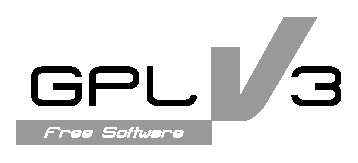
\includegraphics[width=2cm]{gpl-by-christian-candena-cc-by.eps}
\end{flushright}

\vfill\vfill
}

\import{.}{licensing.tex}

\tableofcontents

\import{../00_fp/}{fp-quick-start.tex}
\import{../01_backtrack/}{01_backtrack_main.tex}
%\import{../02_complexity/}{02_complexity_main.tex}
%\import{../03_shortideas/}{03_shortideas_main.tex}
%\import{../04_dfs/}{04_dfs_main.tex}
%\import{../05_dynprog/}{05_dynprog_main.tex}
%\import{../06_testing/}{06_testing_main.tex}
%\import{../07_binsearch/}{07_binsearch_main.tex}

{\makerusother\relax
\immediate\write\tsk{\noexpand\par\noexpand\vspace{0.5cm}\noexpand\epigraph{\noexpand\dotsВы не ужасайтесь\noexpand\dots{} реально все тривиально\noexpand\dots}{}}
}


\inputanswers

\end{document}
